% Options for packages loaded elsewhere
\PassOptionsToPackage{unicode}{hyperref}
\PassOptionsToPackage{hyphens}{url}
%
\documentclass[
]{book}
\title{ReCentering Psych Stats: extRas}
\author{Lynette H. Bikos, PhD, ABPP}
\date{05 Dec 2021}

\usepackage{amsmath,amssymb}
\usepackage{lmodern}
\usepackage{iftex}
\ifPDFTeX
  \usepackage[T1]{fontenc}
  \usepackage[utf8]{inputenc}
  \usepackage{textcomp} % provide euro and other symbols
\else % if luatex or xetex
  \usepackage{unicode-math}
  \defaultfontfeatures{Scale=MatchLowercase}
  \defaultfontfeatures[\rmfamily]{Ligatures=TeX,Scale=1}
\fi
% Use upquote if available, for straight quotes in verbatim environments
\IfFileExists{upquote.sty}{\usepackage{upquote}}{}
\IfFileExists{microtype.sty}{% use microtype if available
  \usepackage[]{microtype}
  \UseMicrotypeSet[protrusion]{basicmath} % disable protrusion for tt fonts
}{}
\makeatletter
\@ifundefined{KOMAClassName}{% if non-KOMA class
  \IfFileExists{parskip.sty}{%
    \usepackage{parskip}
  }{% else
    \setlength{\parindent}{0pt}
    \setlength{\parskip}{6pt plus 2pt minus 1pt}}
}{% if KOMA class
  \KOMAoptions{parskip=half}}
\makeatother
\usepackage{xcolor}
\IfFileExists{xurl.sty}{\usepackage{xurl}}{} % add URL line breaks if available
\IfFileExists{bookmark.sty}{\usepackage{bookmark}}{\usepackage{hyperref}}
\hypersetup{
  pdftitle={ReCentering Psych Stats: extRas},
  pdfauthor={Lynette H. Bikos, PhD, ABPP},
  hidelinks,
  pdfcreator={LaTeX via pandoc}}
\urlstyle{same} % disable monospaced font for URLs
\usepackage{color}
\usepackage{fancyvrb}
\newcommand{\VerbBar}{|}
\newcommand{\VERB}{\Verb[commandchars=\\\{\}]}
\DefineVerbatimEnvironment{Highlighting}{Verbatim}{commandchars=\\\{\}}
% Add ',fontsize=\small' for more characters per line
\usepackage{framed}
\definecolor{shadecolor}{RGB}{248,248,248}
\newenvironment{Shaded}{\begin{snugshade}}{\end{snugshade}}
\newcommand{\AlertTok}[1]{\textcolor[rgb]{0.94,0.16,0.16}{#1}}
\newcommand{\AnnotationTok}[1]{\textcolor[rgb]{0.56,0.35,0.01}{\textbf{\textit{#1}}}}
\newcommand{\AttributeTok}[1]{\textcolor[rgb]{0.77,0.63,0.00}{#1}}
\newcommand{\BaseNTok}[1]{\textcolor[rgb]{0.00,0.00,0.81}{#1}}
\newcommand{\BuiltInTok}[1]{#1}
\newcommand{\CharTok}[1]{\textcolor[rgb]{0.31,0.60,0.02}{#1}}
\newcommand{\CommentTok}[1]{\textcolor[rgb]{0.56,0.35,0.01}{\textit{#1}}}
\newcommand{\CommentVarTok}[1]{\textcolor[rgb]{0.56,0.35,0.01}{\textbf{\textit{#1}}}}
\newcommand{\ConstantTok}[1]{\textcolor[rgb]{0.00,0.00,0.00}{#1}}
\newcommand{\ControlFlowTok}[1]{\textcolor[rgb]{0.13,0.29,0.53}{\textbf{#1}}}
\newcommand{\DataTypeTok}[1]{\textcolor[rgb]{0.13,0.29,0.53}{#1}}
\newcommand{\DecValTok}[1]{\textcolor[rgb]{0.00,0.00,0.81}{#1}}
\newcommand{\DocumentationTok}[1]{\textcolor[rgb]{0.56,0.35,0.01}{\textbf{\textit{#1}}}}
\newcommand{\ErrorTok}[1]{\textcolor[rgb]{0.64,0.00,0.00}{\textbf{#1}}}
\newcommand{\ExtensionTok}[1]{#1}
\newcommand{\FloatTok}[1]{\textcolor[rgb]{0.00,0.00,0.81}{#1}}
\newcommand{\FunctionTok}[1]{\textcolor[rgb]{0.00,0.00,0.00}{#1}}
\newcommand{\ImportTok}[1]{#1}
\newcommand{\InformationTok}[1]{\textcolor[rgb]{0.56,0.35,0.01}{\textbf{\textit{#1}}}}
\newcommand{\KeywordTok}[1]{\textcolor[rgb]{0.13,0.29,0.53}{\textbf{#1}}}
\newcommand{\NormalTok}[1]{#1}
\newcommand{\OperatorTok}[1]{\textcolor[rgb]{0.81,0.36,0.00}{\textbf{#1}}}
\newcommand{\OtherTok}[1]{\textcolor[rgb]{0.56,0.35,0.01}{#1}}
\newcommand{\PreprocessorTok}[1]{\textcolor[rgb]{0.56,0.35,0.01}{\textit{#1}}}
\newcommand{\RegionMarkerTok}[1]{#1}
\newcommand{\SpecialCharTok}[1]{\textcolor[rgb]{0.00,0.00,0.00}{#1}}
\newcommand{\SpecialStringTok}[1]{\textcolor[rgb]{0.31,0.60,0.02}{#1}}
\newcommand{\StringTok}[1]{\textcolor[rgb]{0.31,0.60,0.02}{#1}}
\newcommand{\VariableTok}[1]{\textcolor[rgb]{0.00,0.00,0.00}{#1}}
\newcommand{\VerbatimStringTok}[1]{\textcolor[rgb]{0.31,0.60,0.02}{#1}}
\newcommand{\WarningTok}[1]{\textcolor[rgb]{0.56,0.35,0.01}{\textbf{\textit{#1}}}}
\usepackage{longtable,booktabs,array}
\usepackage{calc} % for calculating minipage widths
% Correct order of tables after \paragraph or \subparagraph
\usepackage{etoolbox}
\makeatletter
\patchcmd\longtable{\par}{\if@noskipsec\mbox{}\fi\par}{}{}
\makeatother
% Allow footnotes in longtable head/foot
\IfFileExists{footnotehyper.sty}{\usepackage{footnotehyper}}{\usepackage{footnote}}
\makesavenoteenv{longtable}
\usepackage{graphicx}
\makeatletter
\def\maxwidth{\ifdim\Gin@nat@width>\linewidth\linewidth\else\Gin@nat@width\fi}
\def\maxheight{\ifdim\Gin@nat@height>\textheight\textheight\else\Gin@nat@height\fi}
\makeatother
% Scale images if necessary, so that they will not overflow the page
% margins by default, and it is still possible to overwrite the defaults
% using explicit options in \includegraphics[width, height, ...]{}
\setkeys{Gin}{width=\maxwidth,height=\maxheight,keepaspectratio}
% Set default figure placement to htbp
\makeatletter
\def\fps@figure{htbp}
\makeatother
\setlength{\emergencystretch}{3em} % prevent overfull lines
\providecommand{\tightlist}{%
  \setlength{\itemsep}{0pt}\setlength{\parskip}{0pt}}
\setcounter{secnumdepth}{5}
\usepackage{booktabs}
\ifLuaTeX
  \usepackage{selnolig}  % disable illegal ligatures
\fi
\usepackage[]{natbib}
\bibliographystyle{plainnat}

\begin{document}
\maketitle

{
\setcounter{tocdepth}{1}
\tableofcontents
}
\hypertarget{book-cover}{%
\chapter*{BOOK COVER}\label{book-cover}}
\addcontentsline{toc}{chapter}{BOOK COVER}

\begin{figure}
\centering
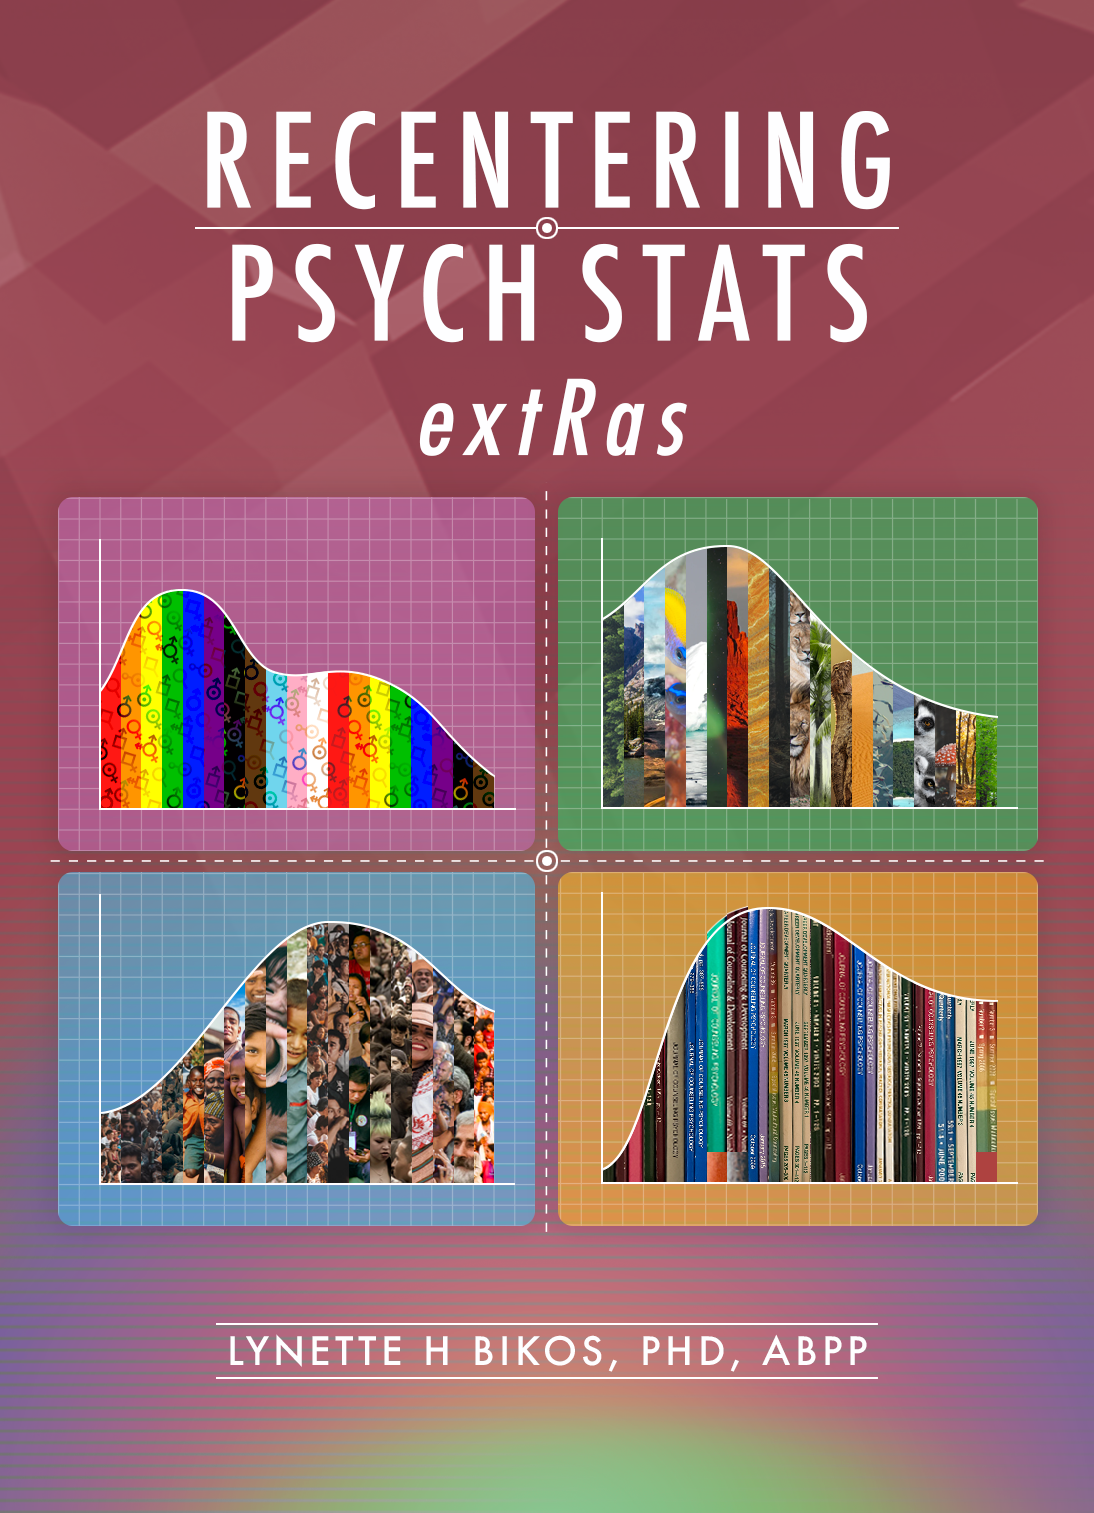
\includegraphics{images/ReCenterPsychStats-extRas-bookcover.png}
\caption{An image of the book cover. It includes four quadrants of non-normal distributions representing gender, race/ethnicty, sustainability/global concerns, and journal articles}
\end{figure}

This open education resource is available in three formats:

\begin{itemize}
\tightlist
\item
  Formatted as an \href{https://lhbikos.github.io/extRas/}{html book} via GitHub Pages
\item
  As a \href{https://github.com/lhbikos/extRas/blob/main/docs/ReC_extRas.pdf}{PDF} available in the \href{https://github.com/lhbikos/extRas/tree/main/docs}{docs} folder at the GitHub repository
\item
  As an \href{https://github.com/lhbikos/extRas/blob/main/docs/ReC_extRas.epub}{ebook} available in the \href{https://github.com/lhbikos/extRas/tree/main/docs}{docs} folder at the GitHub repository
\end{itemize}

All materials used in creating this OER are available at its \href{https://github.com/lhbikos/extRas}{GitHub repo}.

\hypertarget{preface}{%
\chapter*{PREFACE}\label{preface}}
\addcontentsline{toc}{chapter}{PREFACE}

\textbf{If you are viewing this document, you should know that this is a book-in-progress. Early drafts are released for the purpose teaching my classes and gaining formative feedback from a host of stakeholders. The document was last updated on 05 Dec 2021}. Emerging volumes on other statistics are posted on the \href{https://lhbikos.github.io/BikosRVT/ReCenter.html}{ReCentering Psych Stats} page at my research team's website.

\href{https://spu.hosted.panopto.com/Panopto/Pages/Viewer.aspx?id=c932455e-ef06-444a-bdca-acf7012d759a}{Screencasted Lecture Link}

To \emph{center} a variable in regression means to set its value at zero and interpret all other values in relation to this reference point. Regarding race and gender, researchers often center male and White at zero. Further, it is typical that research vignettes in statistics textbooks are similarly seated in a White, Western (frequently U.S.), heteronormative, framework. The purpose of this project is to create a set of open educational resources (OER) appropriate for doctoral and post-doctoral training that contribute to a socially responsive pedagogy -- that is, it contributes to justice, equity, diversity, and inclusion.

Statistics training in doctoral programs are frequently taught with fee-for-use programs (e.g., SPSS/AMOS, SAS, MPlus) that may not be readily available to the post-doctoral professional. In recent years, there has been an increase and improvement in R packages (e.g., \emph{psych}, \emph{lavaan}) used for in analyses common to psychological research. Correspondingly, many graduate programs are transitioning to statistics training in R (free and open source). This is a challenge for post-doctoral psychologists who were trained with other software. This OER will offer statistics training with R and be freely available (specifically in a GitHub respository and posted through GitHub Pages) under a Creative Commons Attribution - Non Commercial - Share Alike license {[}CC BY-NC-SA 4.0{]}.

Training models for doctoral programs in HSP are commonly scholar-practitioner, scientist-practitioner, or clinical-scientist. An emerging model, the \emph{scientist-practitioner-advocacy} training model incorporates social justice advocacy so that graduates are equipped to recognize and address the sociocultural context of oppression and unjust distribution of resources and opportunities \citep{mallinckrodt_scientist-practitioner-advocate_2014}. In statistics textbooks, the use of research vignettes engages the learner around a tangible scenario for identifying independent variables, dependent variables, covariates, and potential mechanisms of change. Many students recall examples in Field's \citeyearpar{field_discovering_2012} popular statistics text: Viagra to teach one-way ANOVA, beer goggles for two-way ANOVA, and bushtucker for repeated measures. What if the research vignettes were more socially responsive?

In this OER, research vignettes will be from recently published articles where:

\begin{itemize}
\tightlist
\item
  the author's identity is from a group where scholarship is historically marginalized (e.g., BIPOC, LGBTQ+, LMIC{[}low-middle income countries{]}),
\item
  the research is responsive to issues of justice, equity, inclusion, diversity,
\item
  the lesson's statistic is used in the article, and
\item
  there is sufficient information in the article to simulate the data for the chapter example(s) and practice problem(s); or it is publicly available.
\end{itemize}

In training for multicultural competence, the saying, ``A fish doesn't know that it's wet'' is often used to convey the notion that we are often unaware of our own cultural characteristics. In recent months and years, there has been an increased awakening to the institutional and systemic racism that our systems are perpetuating. Queuing from the water metaphor, I am hopeful that a text that is recentered in the ways I have described can contribute to \emph{changing the water} in higher education and in the profession of psychology.

\hypertarget{copyright-with-open-access}{%
\section*{Copyright with Open Access}\label{copyright-with-open-access}}
\addcontentsline{toc}{section}{Copyright with Open Access}

This book is published under a a Creative Commons Attribution-NonCommercial-ShareAlike 4.0 International License. This means that this book can be reused, remixed, retained, revised and redistributed (including commercially) as long as appropriate credit is given to the authors. If you remix, or modify the original version of this open textbook, you must redistribute all versions of this open textbook under the same license - CC BY-SA.

A \href{https://github.com/lhbikos/ReC_Psychometrics}{GitHub open-source repository} contains all of the text and source code for the book, including data and images.

\hypertarget{acknowledgements}{%
\chapter*{ACKNOWLEDGEMENTS}\label{acknowledgements}}
\addcontentsline{toc}{chapter}{ACKNOWLEDGEMENTS}

As a doctoral student at the University of Kansas (1992-2005), I learned that ``a foreign language'' was a graduation requirement. \emph{Please note that as one who studies the intersections of global, vocational, and sustainable psychology, I regret that I do not have language skills beyond English.} This could have been met with credit from high school my rural, mid-Missouri high school did not offer such classes. This requirement would have typically been met with courses taken during an undergraduate program -- but my non-teaching degree in the University of Missouri's School of Education was exempt from this. The requirement could have also been met with a computer language (fortran, C++) -- I did not have any of those either. There was a tiny footnote on my doctoral degree plan that indicated that a 2-credit course, ``SPSS for Windows'' would substitute for the language requirement. Given that it was taught by my one of my favorite professors, I readily signed up. As it turns out, Samuel B. Green, PhD, was using the course to draft chapters in the textbook \citep{green_using_2014} that has been so helpful for so many. Unfortunately, Drs. Green (1947 - 2018) and Salkind (2947 - 2017) are no longer with us. I have worn out numerous versions of their text. Another favorite text of mine was Dr.~Barbara Byrne's \citeyearpar{byrne_structural_2016}, ``Structural Equation Modeling with AMOS.'' I loved the way she worked through each problem and paired it with a published journal article, so that the user could see how the statistical evaluation fit within the larger project/article. I took my tea-stained text with me to a workshop she taught at APA and was proud of the signature she added to it (a little catfur might have fallen out). Dr.~Byrne created SEM texts for a number of statistical programs (e.g., LISREL, EQS, MPlus). As I was learning R, I wrote Dr.~Byrne, asking if she had an edition teaching SEM/CFA with R. She promptly wrote back, saying that she did not have the bandwidth to learn a new statistics package. We lost Dr.~Byrne in December 2020. I am so grateful to these role models for their contributions to my statistical training. I am also grateful for the doctoral students who have taken my courses and are continuing to provide input for how to improve the materials.

The inspiration for training materials that re*center statistics and research methods came from the \href{https://www.academics4blacklives.com/}{Academics for Black Survival and Wellness Initiative}. This project, co-founded by Della V. Mosley, Ph.D., and Pearis L. Bellamy, M.S., made clear the necessity and urgency for change in higher education and the profession of psychology.

At very practical levels, I am indebted to SPU's Library, and more specifically, SPU's Education, Technology, and Media Department. Assistant Dean for Instructional Design and Emerging Technologies, R. John Robertson, MSc, MCS, has offered unlimited consultation, support, and connection. Senior Instructional Designer in Graphics \& Illustrations, Dominic Wilkinson, designed the logo and bookcover. Psychology and Scholarly Communications Librarian, Kristin Hoffman, MLIS, has provided consultation on topics ranging from OERS to citations. I am alo indebted to Associate Vice President, Teaching and Learning at Kwantlen Polytechnic University, Rajiv Jhangiani, PhD. Dr.~Jhangiani's text \citeyearpar{jhangiani_research_2019} was the first OER I ever used and I was grateful for his encouraging conversation.

Financial support for this project has been provided the following:

\begin{itemize}
\tightlist
\item
  \emph{Call to Action on Equity, Inclusion, Diversity, Justice, and Social Responsivity Request for Proposals} grant from the Association of Psychology Postdoctoral and Internship Centers (2021-2022).
\item
  \emph{Diversity Seed Grant}, Office of Inclusive Excellence and Advisory Council for Diversity and Reconciliation (ACDR), Seattle Pacific University.
\item
  \emph{ETM Open Textbook \& OER Development Funding}, Office of Education, Technology, \& Media, Seattle Pacific University.
\end{itemize}

\hypertarget{the-mechanics-behind-recentering}{%
\chapter*{THE MECHANICS BEHIND RECENTERING}\label{the-mechanics-behind-recentering}}
\addcontentsline{toc}{chapter}{THE MECHANICS BEHIND RECENTERING}

\hypertarget{book1}{%
\chapter{\texorpdfstring{From \emph{bookdown} to GitHub Pages}{From bookdown to GitHub Pages}}\label{book1}}

\href{https://spu.hosted.panopto.com/Panopto/Pages/Viewer.aspx?pid=7c20cc56-069a-40e2-abc7-adf3017f8c47}{Screencast Link}

\emph{ReCentering Psych Stats} volumes are all created with a combination of R, R Studio, bookdown (the package), the GitHub, GitHub Desktop, GitHub Pages, and a host of packages. There is abundant information on all of these tools across the internet. In this lesson, I walk through the steps in creating the templated \href{https://bookdown.org/}{bookdown} ``book'' using Yihui Xie's \emph{bookdown} package and processes. Two regularly updated sources \citep{xie_authoring_2021, xie_r_2021} provide a strong foundation to this process. Additionally, a quick internet search will yield additional resources for examples, unique circumstances, and idea generation. At the outset, please know that the instructions I provide is based on my experience with my projects and the work that we do in my research team. It is quite possible they will not be as applicable in other contexts.

As I have continued in this journey of learning R, teaching R, and creating an open education resource, I have consulted and relied upon many resources beyond. Visiting the GitHub repository of two resources have been especially useful in gaining these skills. After struggling to comprehend some of the instructions in the \emph{bookdown} source materials I happened upon a chapter in Dougherty's, \href{https://ontheline.trincoll.edu/}{On The Line: How Schooling, Housing, and Civil Rights Shaped Hartford and its Suburbs}. I was first drawn to a closing chapter in this open-access digital book that described Dougherty's \citeyearpar{dougherty_chapter_2021} use of \emph{bookdwn}, the GitHub, and GitHub pages. When I realized that this project was entirely available on a \href{https://github.com/OnTheLine/otl-bookdown}{GitHub repo}, I learned that I could visit, inspect, and clone (i.e., make a copy of the GitHub repository) of this project. Soon after, I also learned that Navarro's \citep{navarro_book_2020} \href{https://learningstatisticswithr.com/}{Learning Statistics with R} was also available in a \href{https://github.com/djnavarro/rbook}{GitHub repo}. Together, the original R Markdown and bookdown training materials plus the two enacted examples were a tremendous resources of potential solutions I could try. For example, on one frustrating day, I could not get my book to build. I cloned Dougherty's OTL, opened his project on my laptop, and asked the project to build. When it did (flawlessly), I copied and adapted his code (I recall my struggles were in the YAML matter atop the index.rmd) until I could get my project to work. Until very recently, you could still see ``otl'' references in hashtagged out lines of code in some of the early volumes of ReCentering.

\emph{Note. If you are at an institution like mine and you have an enterprise-issued computer it may matter whether your R projects are on your local drive or a cloud-drive. At SPU it is possible to use R Studio with .rmd files and such on the local drive. But they will only knit if the projects are on the OneDrive directory.}

\hypertarget{creating-a-bookdown-template}{%
\section{\texorpdfstring{Creating a \emph{bookdown} template}{Creating a bookdown template}}\label{creating-a-bookdown-template}}

Before beginning the process, make sure you have installed bookdown:

\begin{Shaded}
\begin{Highlighting}[]
\CommentTok{\#install.packages("bookdown", dependencies = T)}
\end{Highlighting}
\end{Shaded}

Additionally, know in advance where (i.e., the parent folder) you want the book to be located. With this in mind:

\begin{enumerate}
\def\labelenumi{\arabic{enumi}.}
\tightlist
\item
  Open R Studio
\item
  Under the ``File'' menu select

  \begin{itemize}
  \tightlist
  \item
    New Project (if prompted, you do not need to save the workspace image, although you may wish to save any files that you have worked on)
  \item
    New Directory
  \item
    Book project using \emph{bookdown}
  \end{itemize}
\item
  In the New Project Wizard

  \begin{itemize}
  \tightlist
  \item
    The ``Directory name'' will be both the project name and the name of the folder that houses all the bookdown parts and pieces. In my example ``xtRas'' is what I entered in ``Directory name.''
  \item
    Use the ``Browse'' button to navigate to the parent folder. In my example, I selected ``C/Users/myaccount/OneDrive - InstitutionName/ReCenterPsychStats''
  \item
    Create Project
  \end{itemize}
\end{enumerate}

Once created, your project folder will be pre-populated with a number of objects that will serve as tutorials and templates for your work.

\hypertarget{establishing-an-output-directory-needed-to-publish-on-github-pages}{%
\section{Establishing an Output Directory (needed to publish on GitHub Pages)}\label{establishing-an-output-directory-needed-to-publish-on-github-pages}}

If your goal is to present your book through the free webpages of GitHub Pages it is necessary to update some yml matter. Specifically, navigate to the ``\_bookdown.yml'' and edit it by adding script that will route the webpages (and their structure) to a folder titled ``docs''. In total, the entirety of script in my ``\_bookdown.yml'' is this:

book\_filename: ``ReC\_extRas''
delete\_merged\_file: true
language:
ui:
chapter\_name: ``Chapter''
output\_dir: ``docs''

\hypertarget{the-index.rmd-file-is-first}{%
\section{\texorpdfstring{The \emph{index.Rmd} File is First}{The index.Rmd File is First}}\label{the-index.rmd-file-is-first}}

In this section of the tutorial, I navigate to the ``index.Rmd'' file and merely change the .yml matter related to the title and author so that when we render the book to GitHub Pages we can see that it was, in fact, this project that was rendered.

\hypertarget{build-the-book}{%
\section{Build the Book!}\label{build-the-book}}

To build the book select the ``Build'' tab from the upper right hand box in R Studio. Within that tab, select ``Build Book.'' You can find the rendered book in the docs folder (which it created automatically if you added the command to the *\_bookdown.yml* file). Select any of the html files and it will show you the built book.

\hypertarget{send-it-to-the-github}{%
\section{Send it to the GitHub}\label{send-it-to-the-github}}

Using the GitHub Pages means that you also have a \href{https://github.com}{GitHub} account. If you haven't already, register for an account. Additionally, make sure to download, install and open \href{https://desktop.github.com/}{GitHub Desktop}.

Very briefly (because there is so much more), the GitHub is an open source community where you can (freely) create repositories and collaborate on them. The GitHub Desktop allows you to clone your repositories to your local environment, work on them, and then update the GitHub repository. In our case, we are starting with the bookdown R project on our local computer and turning it into a GitHub Repository. From this GitHub repo, it will be pushed to GitHub Pages.

\begin{enumerate}
\def\labelenumi{\arabic{enumi}.}
\tightlist
\item
  Open GitHub Desktop
\item
  Under the ``File'' menu, select

  \begin{itemize}
  \tightlist
  \item
    Add local repository
  \item
    With the ``Choose'' tool, navigate to the the folder that holds the bookdown project (in my case it was ``extRas'')
  \item
    GitHub Desktop is smart and recognizes that it is not a Git repository. For now it has been working for me to select ``create a repository'' and use the GitHub Desktop defaults
  \end{itemize}
\item
  Selct ``Publish repository''

  \begin{itemize}
  \tightlist
  \item
    Optional to add a description
  \end{itemize}
\end{enumerate}

\hypertarget{publish-on-github-pages}{%
\section{Publish on GitHub Pages}\label{publish-on-github-pages}}

Publishing the bookdown project to GitHub pages implies that you have aleady changed the ``\_bookdown.yml'' script to include the \emph{output\_dir: ``docs''}

Select ``Settings.'' Scroll to the bottom, to the ``Danger Zone'' to make sure that the repository is public. If not, select ``Change visibility'' and select ``Make Public.''

Still in settings, select ``Pages'' (menu bar on left).

\begin{itemize}
\tightlist
\item
  Under ``Source'' select:

  \begin{itemize}
  \tightlist
  \item
    Branch: main
  \item
    /docs
  \item
    save
  \end{itemize}
\end{itemize}

After a few minutes, your webpage will be available at the website that was provided on the setup for GitHub Pages. It will look like: \url{https:/YOURACCOUNT.github.io/YOURPROJECT/}

\hypertarget{updating-via-github-desktop}{%
\section{Updating via GitHub Desktop}\label{updating-via-github-desktop}}

\emph{Perpetually in progress} texts are continuously updated. When you have updates

\begin{itemize}
\tightlist
\item
  Open GitHub Desktop
\item
  Navigate to the repository

  \begin{itemize}
  \tightlist
  \item
    Use the dropdown menu under Current respository (upper left of app)
  \end{itemize}
\item
  If there are changes in the left panel then an update is appropriate; if there are none, nothing will update.
\item
  Brief text is required in the ``Summary'' box (lower left)

  \begin{itemize}
  \tightlist
  \item
    It is optional to provide a description. I often leave cryptic summaries and no description. If, however, there was something significant/meaningful, I would elaborate more.
  \end{itemize}
\item
  Click ``Commit to main''
\item
  Click ``Push origin'' found either in the center of the menu bar or in the middle of the page.
\end{itemize}

That's it! Depending on the size of the project/changes, all of the documents in the GitHub Repo and the GitHub Pages repo book will be updated. From time-to-time you may wish to cull the GitHub repo to remove older documents that may have been created but replaced (because of renaming or something) and are no longer in use.

\hypertarget{pdf-and-epub-compilations}{%
\section{PDF and epub Compilations}\label{pdf-and-epub-compilations}}

It has taken me quite some time to figure out compilation as a PDF. There seem to be a couple of elements that make it successful. First, it is essential to have the tinytex package installed. Use this two-part code:

\begin{Shaded}
\begin{Highlighting}[]
\CommentTok{\#install.packages(\textquotesingle{}tinytex\textquotesingle{})}
\CommentTok{\#tinytex::install\_tinytex()}
\end{Highlighting}
\end{Shaded}

Second, inspect the ``\_output.yml'' content.

\begin{Shaded}
\begin{Highlighting}[]
\NormalTok{bookdown}\SpecialCharTok{::}\NormalTok{gitbook}\SpecialCharTok{:}
\NormalTok{  css}\SpecialCharTok{:}\NormalTok{ style.css}
\NormalTok{  config}\SpecialCharTok{:}
\NormalTok{    toc}\SpecialCharTok{:}
\NormalTok{      before}\SpecialCharTok{:} \ErrorTok{|}
        \ErrorTok{\textless{}}\NormalTok{li}\SpecialCharTok{\textgreater{}}\ErrorTok{\textless{}}\NormalTok{a href}\OtherTok{=}\StringTok{"./"}\SpecialCharTok{\textgreater{}}\NormalTok{ReCentering Psych Stats extRas}\SpecialCharTok{\textless{}}\ErrorTok{/}\NormalTok{a}\SpecialCharTok{\textgreater{}}\ErrorTok{\textless{}/}\NormalTok{li}\SpecialCharTok{\textgreater{}}
\NormalTok{      after}\SpecialCharTok{:} \ErrorTok{|}
        \ErrorTok{\textless{}}\NormalTok{li}\SpecialCharTok{\textgreater{}}\ErrorTok{\textless{}}\NormalTok{a href}\OtherTok{=}\StringTok{"https://github.com/rstudio/bookdown"}\NormalTok{ target}\OtherTok{=}\StringTok{"blank"}\SpecialCharTok{\textgreater{}}\NormalTok{Published with bookdown}\SpecialCharTok{\textless{}}\ErrorTok{/}\NormalTok{a}\SpecialCharTok{\textgreater{}}\ErrorTok{\textless{}/}\NormalTok{li}\SpecialCharTok{\textgreater{}}
\NormalTok{    edit}\SpecialCharTok{:}\NormalTok{ https}\SpecialCharTok{:}\ErrorTok{//}\NormalTok{github.com}\SpecialCharTok{/}\NormalTok{USERNAME}\SpecialCharTok{/}\NormalTok{REPO}\SpecialCharTok{/}\NormalTok{edit}\SpecialCharTok{/}\NormalTok{BRANCH}\SpecialCharTok{/}\NormalTok{\%s}
\NormalTok{    download}\SpecialCharTok{:}\NormalTok{ [}\StringTok{"pdf"}\NormalTok{, }\StringTok{"epub"}\NormalTok{]}
\NormalTok{bookdown}\SpecialCharTok{::}\NormalTok{pdf\_book}\SpecialCharTok{:}
\NormalTok{  includes}\SpecialCharTok{:}
\NormalTok{    in\_header}\SpecialCharTok{:}\NormalTok{ preamble.tex}
\NormalTok{  latex\_engine}\SpecialCharTok{:}\NormalTok{ xelatex}
\NormalTok{  citation\_package}\SpecialCharTok{:}\NormalTok{ natbib}
\NormalTok{  keep\_tex}\SpecialCharTok{:}\NormalTok{ yes}
\NormalTok{bookdown}\SpecialCharTok{::}\NormalTok{epub\_book}\SpecialCharTok{:}\NormalTok{ default}
\end{Highlighting}
\end{Shaded}

As you can see, the default instructions from the \emph{bookdown} template include both pdf and epub formats. You can retrieve them from the docs folder.

\hypertarget{formatting-the-book}{%
\chapter{Formatting the Book}\label{formatting-the-book}}

\href{https://spu.hosted.panopto.com/Panopto/Pages/Viewer.aspx?pid=430263b6-f1bd-4a8c-a393-adf501447448}{Screencast Link}

In this lesson I review the formatting tools and conventions that I use most often. This is not an exhaustive list of formatting tools, just the ones that have been useful in the \emph{ReCentering Psych Stats} project. If you haven't found them already, do check out the two regularly updated official documentation for using R Markdown with \emph{bookdown} \citep{xie_authoring_2021, xie_r_2021}.

The \emph{bookdown} project has a very specific file structure. The \emph{index.Rmd} file must be first and must have that exact name (i.e., ``index.Rmd''). The files that follow should be numbered in the order in which you want them to appear. While you may wish to give each chapter its unique number, the \emph{bookdown} packages numbers the chapters by the single hashtag -- skipping over any that have the dash (enclosed in squiggly parentheses). That is, the numbers associated with each of the .Rmd files may not correspond with chapter numbers unless you have carefully hashtagged out some of the single hashtags.

Let's start by exploring the \emph{index.Rmd}

\hypertarget{the-yaml-matter-atop-the-index.rmd}{%
\section{\texorpdfstring{The YAML matter atop the \emph{index.Rmd}}{The YAML matter atop the index.Rmd}}\label{the-yaml-matter-atop-the-index.rmd}}

The material at the top of the \emph{index.Rmd} is often called ``yaml matter'' (``Yet Another Markup Language'') and provides instructions for how the document is to be rendered. These instructions appear between three dashed lines before and after the YAML header.

In decoding what is and is not necessary in my YAML header (and learning what each command does), I have often visited other open source documents such as Dougherty's \citeyearpar{dougherty_chapter_2021} \href{https://github.com/OnTheLine/otl-bookdown}{On the Line} and Navarro's \citeyearpar{navarro_book_2020} \href{https://github.com/djnavarro/rbook}{Learning Statistics with R} which are both available GitHub (the links are to their GitHub repos). The text below is what is in the YAML of this index.

The sections of highlighted text below are copied directly from the YAML header in this mini-volume. Most of it will seem self-explanatory. However, I offer brief explanations following sections of the script. If you access the .rmd file itself, I left left some of these clues using by commenting them out with hashtags.

\begin{Shaded}
\begin{Highlighting}[]
\NormalTok{title}\SpecialCharTok{:} \StringTok{"ReCentering Psych Stats: extRas"}
\NormalTok{author}\SpecialCharTok{:} \StringTok{"Lynette H. Bikos, PhD, ABPP"}
\NormalTok{date}\SpecialCharTok{:} \StringTok{"\textasciigrave{}r format (Sys.Date(), \textquotesingle{}\%d \%b \%Y\textquotesingle{})\textasciigrave{}"}
\end{Highlighting}
\end{Shaded}

Title and date are likely obvious. When the date, entered following ``r'' (using the format: `\texttt{r} `) the date at the time of the knit or build will auto-update, like this: 05 Dec 2021. As might be obvious from the ``format'' and ``\%d \%b \%Y'' code, the date can be presented in a variety of structures. More instructions are available in the R Markdown Cookbook \citep{xie_r_2021}.

\begin{Shaded}
\begin{Highlighting}[]
\NormalTok{site}\SpecialCharTok{:}\NormalTok{ bookdown}\SpecialCharTok{::}\NormalTok{bookdown\_site}
\NormalTok{documentclass}\SpecialCharTok{:}\NormalTok{ book}
\end{Highlighting}
\end{Shaded}

The site and document class commands (and their settings) are the defaults in the bookdown template. They allow RStudio to recognize the directory as a book source directory and it will add the ``Build Book'' button in the ``Build'' pane \citep{xie_r_2021}.

\begin{Shaded}
\begin{Highlighting}[]
\NormalTok{citation}\SpecialCharTok{{-}}\NormalTok{style}\SpecialCharTok{:}\NormalTok{ apa}\SpecialCharTok{{-}}\NormalTok{single}\SpecialCharTok{{-}}\NormalTok{spaced.csl }\CommentTok{\#}
\NormalTok{bibliography}\SpecialCharTok{:}\NormalTok{ STATSnMETH.bib }
\NormalTok{link}\SpecialCharTok{{-}}\NormalTok{citations}\SpecialCharTok{:}\NormalTok{ yes}
\end{Highlighting}
\end{Shaded}

There are a variety of citation styles. I changed the default to the style for the 7th edition of the APA Style Manual. You will need to download this style sheet and put a copy in the project folder. Of course you can copy and use mine, or you can obtain a fresh copy at the \href{https://www.zotero.org/styles}{Zotero Style Repository}. There you can find more than 10,000 styles -- including at least eight versions of the 7th edition of the APA Style manual!

The style sheet is essential if you include references. I use Zotero and ensure that all the references that I cite are included in a project-specific folder. From Zotero, I export (by right-clicking) that folder in the BibTex format (selecting ``Export Notes'') to the project folder. Any time I add references or update the formatting of any of the Zotero entries, I must re-export the folder to my bookdown project folder and restart R. Your reference folder can have any name that you give it.

Finally, specifying ``yes'' to the ``link-citations'' command will render live links to the citations that Zotero (or your reference manager) provides.

All of these appear to be optional; the book will render without them. If you are not planning to use citations, you can hashtag them out (keeping them as placeholders for potential use later) or delete them altogether.

\begin{Shaded}
\begin{Highlighting}[]
\NormalTok{url}\SpecialCharTok{:}\NormalTok{ https}\SpecialCharTok{:}\ErrorTok{//}\NormalTok{lhbikos.github.io}\SpecialCharTok{/}\NormalTok{extRas}\SpecialCharTok{/} 
\NormalTok{cover}\SpecialCharTok{{-}}\NormalTok{image}\SpecialCharTok{:}\NormalTok{ images}\SpecialCharTok{/}\NormalTok{ReCenterPsychStats}\SpecialCharTok{{-}}\NormalTok{extRas}\SpecialCharTok{{-}}\NormalTok{bookcover.png }
\NormalTok{description}\SpecialCharTok{:} \ErrorTok{|}
  \StringTok{"extRas"}\NormalTok{ is a mini}\SpecialCharTok{{-}}\NormalTok{volume }\ControlFlowTok{in}\NormalTok{ the ReCentering Psych Stats series that is devoted to some of the technical tools and processes used that just do not fit easily }\ControlFlowTok{in}\NormalTok{ the regular }\FunctionTok{volumes}\NormalTok{ (e.g., ANOVA, psychometrics, multivariate). The examples and instructions may be somewhat limiting }\ControlFlowTok{in}\NormalTok{ that they have a specific use}\SpecialCharTok{{-}}\NormalTok{case }\ControlFlowTok{for}\NormalTok{ graduate students }\ControlFlowTok{in}\NormalTok{ psychology programs at our institution.}
\NormalTok{github}\SpecialCharTok{{-}}\NormalTok{repo}\SpecialCharTok{:}\NormalTok{ lhbikos}\SpecialCharTok{/}\NormalTok{extRas}
\end{Highlighting}
\end{Shaded}

Although I am not presently seeing where these are being utilized, I went with the defaults, adding my own url, cover-image, description, and specification to the GitHub repository. These appear to be optional; the book will render without them. If you are not planning to use citations, you can hashtag them out (keeping them as placeholders for potential use later) or delete them altogether.

If you include the description, make sure to keep the pipe (\textbar) that occurs immediately after the command.

\hypertarget{my-go-to-formatting-tools}{%
\section{My Go-To Formatting Tools}\label{my-go-to-formatting-tools}}

R Markdown and bookdown offer a number of options for formatting text. My purpose is to merely provide an introduction to the techniques that I have used most frequently in ReCentering Psych Stats. Not surprisingly, there are tremendous resources on the internet that provide instruction and examples. A helpful second stop beyond my resource is Chapter 5 (Formatting) of the R Markdown Cookbook \citep{xie_r_2021} and Authoring Books with R Markdown \citep{xie_r_2021}.

\hypertarget{chapter-numbering}{%
\subsection{Chapter numbering}\label{chapter-numbering}}

Bookdown treats the single hashtag as a chapter and, by default (this can be changed) will number accordingly. I have used the \emph{index.Rmd} to host a PREFACE and ACKNOWLEDGEMENTS I have sectioned these with a single hashtag, but because I added the ``\{-\}'' symbol, they are not treated as numbers and not included in the numbering system. An example of this is THE MECHANICS BEHIND RECENTERING section, which includes several chapters devoted to the integration of bookdown, GitHub, GitHub Pages. My own convention is to use ALL CAPS when I am including a significant section that is not considered to be a numbered chapter.

There needs to be a line space before and after each use of the chapter heading. If you would like to provide a nickname that you can use later to cross-reference back to this chapter or section, include a hashtag and nickname in the squiggly parentheses.

Subheadings are created by adding additional hashtags. Specificaly, two hashtags (\#\#) is subordinate to the chapter level heading (we'll call it the parent heading) and three hashtags (\#\#\#) are the child-heading to the parent.

\begin{Shaded}
\begin{Highlighting}[]
\CommentTok{\# UNNUMBERED CHAPTER HEADING \{{-}\}}

\CommentTok{\# Chapter Heading Numbered with Cross{-}Reference Link \{\#chapterlink\}}

\DocumentationTok{\#\# Subheading (parent)}

\DocumentationTok{\#\#\# Subheading (child)}
\end{Highlighting}
\end{Shaded}

\begin{Shaded}
\begin{Highlighting}[]
\NormalTok{Later, I can can provide a link that will cross}\SpecialCharTok{{-}}\NormalTok{reference back to the [Chapter](}\CommentTok{\#chapterlink).}
\end{Highlighting}
\end{Shaded}

Here is a functional example linking back to the \protect\hyperlink{book1}{From \emph{bookdown} to GitHub Pages} chapter.

\hypertarget{bulleted-and-numbered-lists}{%
\subsection{Bulleted and numbered lists}\label{bulleted-and-numbered-lists}}

My understanding that when books are written for use on the internet short(er) paragraphs and lists can be helpful to the reader in that they reduce the cognitive load.

Bulleted lists can be specified with the '*' , `-'```, or'+' signs, interchangeably. For no specific reason, I often use the asterisk for parent-level headings and a dash for child-level headings. A line space is required between the text above the first bullet.

\begin{Shaded}
\begin{Highlighting}[]
\NormalTok{If I am going to make a bulleted list I will start by leaving a space between the text and the first item }\ControlFlowTok{in}\NormalTok{ the list}\SpecialCharTok{:}

\ErrorTok{*}\NormalTok{ Parent item }\DecValTok{1}
\SpecialCharTok{*}\NormalTok{ Parent item }\DecValTok{2}
  \SpecialCharTok{{-}}\NormalTok{ Child item }\DecValTok{1}
  \SpecialCharTok{{-}}\NormalTok{ Child item }\DecValTok{2}
\end{Highlighting}
\end{Shaded}

The rendered result is this. If I am going to make a bulleted list I will start by leaving a space between the text and the first item in the list:

\begin{itemize}
\tightlist
\item
  Parent item 1
\item
  Parent item 2

  \begin{itemize}
  \tightlist
  \item
    Child item 1
  \item
    Child item 2
  \end{itemize}
\end{itemize}

At times you may wish to have numbered lists. The structure is the same.

\begin{Shaded}
\begin{Highlighting}[]
\NormalTok{If I am going to make a numbered list I will start by leaving a space between the text and the first item }\ControlFlowTok{in}\NormalTok{ the list}\SpecialCharTok{:}
  
\FloatTok{1.}\NormalTok{ Parent item }\DecValTok{1}
\FloatTok{2.}\NormalTok{ Parent item }\DecValTok{2}
   \SpecialCharTok{{-}}\NormalTok{ Child item }\DecValTok{1}
   \SpecialCharTok{{-}}\NormalTok{ Child item }\DecValTok{2}
\end{Highlighting}
\end{Shaded}

The rendered result is this. If I am going to make a numbered list I will start by leaving a space between the text and the first item in the list:

\begin{enumerate}
\def\labelenumi{\arabic{enumi}.}
\tightlist
\item
  Parent item 1
\item
  Parent item 2

  \begin{itemize}
  \tightlist
  \item
    Child item 1
  \item
    Child item 2
  \end{itemize}
\end{enumerate}

\hypertarget{text-emphasis}{%
\subsection{Text emphasis}\label{text-emphasis}}

Emphasizing text can be helpful in conveying the meaning in the finished document. My understanding is that we should use the built-in systems (in the case of bookdown, using the \# system for headings/subheadings) for the heading structure. This is so that text-readers will recognize and emphasize appropriately. I have also understood that underlining is discouraged because it may give the impression that there is a hyperlink. Therefore my go-to's are \emph{italics} and \textbf{bold}.

\emph{Italics} is created by placing a single asterisk around the intended word or phrase; \textbf{bold} is created with a double asterisk around the word or phrase to be bolded. This sentence is demonstrated, below.

\begin{Shaded}
\begin{Highlighting}[]
\SpecialCharTok{*}\NormalTok{Italics}\SpecialCharTok{*}\NormalTok{ is created by placing a single asterisk around the intended sired word or phrase; }\SpecialCharTok{**}\NormalTok{bold}\SpecialCharTok{**}\NormalTok{ is created with a double asterisk around the word or phrase to be bolded.}
\end{Highlighting}
\end{Shaded}

By now you may have noticed that the asterisk can be uses for bulleted lists, italics, and bold. Yes, there will be times when R will read the asterisks in a confusing way and you will need to think careful about the coding and how to order it.

There are times when I want emphasize something in the text with \texttt{highlights} rather than with \emph{italics} or \textbf{bold}. This is possible by surrounding the words with tic (```'') marks. This sentence is repeated below to demonstrate the different techniques.

\begin{Shaded}
\begin{Highlighting}[]
\NormalTok{There are times when I want emphasize something }\ControlFlowTok{in}\NormalTok{ the text with }\StringTok{\textasciigrave{}}\AttributeTok{highlights}\StringTok{\textasciigrave{}}\NormalTok{ rather than with }\SpecialCharTok{*}\NormalTok{italics}\SpecialCharTok{*}\NormalTok{ (surrounding the tet }\ControlFlowTok{in}\NormalTok{ single asterisks) or }\SpecialCharTok{**}\NormalTok{bold}\SpecialCharTok{**}\NormalTok{ (surrounding the text }\ControlFlowTok{in}\NormalTok{ double asterisks.}
\end{Highlighting}
\end{Shaded}

If I want to highlight an entire section, I enter a code chunk and then in the chunk header write ``r eval=FALSE''. The command, ``eval=FALSE'' means that R will simply print what is in the chunk, but not try to execute it. This results in the boxes of highlights that you see. Unfortunately, I have not figured out a way to show this in a highlighted box. Note that text does not wrap automatically in these chunks, this is why a slider appears on the bottom of some of these chunks. Returns (ENTER) can help with spacing if you prefer.

\hypertarget{adding-images}{%
\subsection{Adding images}\label{adding-images}}

Images can be critical in conveying important messages and I use them abundantly. My strategy has been to store an image in the project folder (usually in a chapter folder in an images folder in the project folder) and then call it with the code below. Note that the code allows for a figure caption. Another principle of universal design is to provide text captions.

Before uploading the imagine, I created a single image (from the four photos) and saved it as a .png. With very little sophistication, I used the Snip \& Sketch app on my Windows machine and the picture tools in Microsoft Word. The photos were taken by Shari Young Kuchenbecker, PhD, and were part of the official post-convention collection that were posted at the \href{https://westernpsych.org/2018-convention-photos/}{WPA Convention Site}. The story behind the photos is that my then-advisee, Desta Gebregiorgis (now Dr.~Gebregiorgis), and I were receiving an awesome stats consult from the quantiative psychologist Jodie Ullman, PhD, a Professor at the California State University, San Bernardino. As evidenced in the increasingly perplexed facial expressions, it was complicated.

\begin{Shaded}
\begin{Highlighting}[]
\SpecialCharTok{!}\NormalTok{[A four}\SpecialCharTok{{-}}\NormalTok{photo series of thumbnails depicting three individuals sitting around a table trying to solve a statistics dilemma. The facial expressions become increasingly bewildered across the series.](images}\SpecialCharTok{/}\NormalTok{formatting}\SpecialCharTok{/}\NormalTok{StatsConsult.png)}
\end{Highlighting}
\end{Shaded}

\begin{figure}
\centering
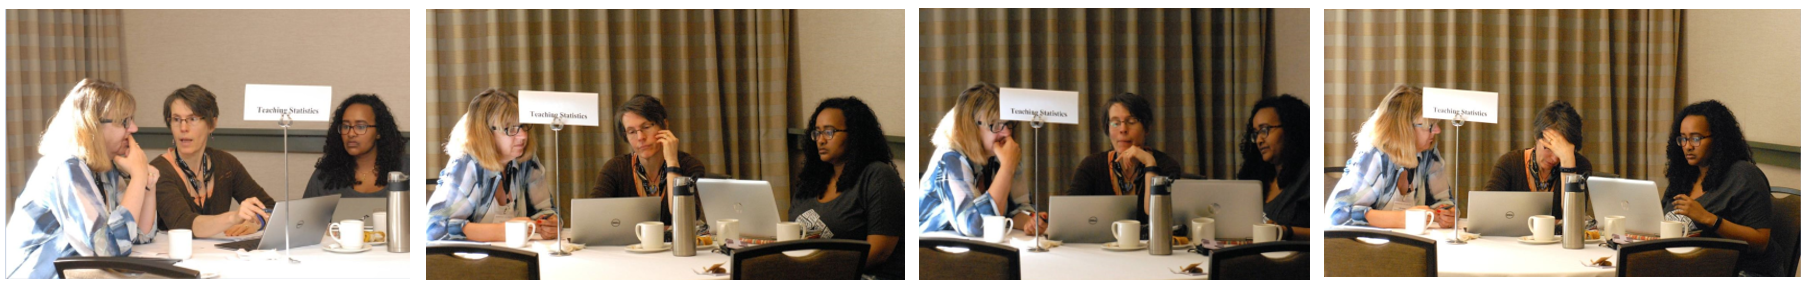
\includegraphics{images/formatting/StatsConsult.png}
\caption{A four-photo series of thumbnails depicting three individuals sitting around a table trying to solve a statistics dilemma. The facial expressions become increasingly bewildered across the series.}
\end{figure}

\hypertarget{creating-a-table-from-within-the-.rmd-file}{%
\subsection{Creating a table from within the .rmd file}\label{creating-a-table-from-within-the-.rmd-file}}

Often times we will use packages to create, present, and imbed tables and figures as we conduct the statistical analysis. At other times, we may wish to create a table without an external dataset. I do this in nearly every ReCentering Psych Stats chapter when I create the grading rubric. At other times, I may create a table to facilitate comprehension of a statistical concept. Here is a the classic table used to convey the relationship between Type I and Type II error.

Here's the code for producing the table (actually two distinct tables) that follows. The specification is simultaneously simple and complex. Several guidelines will help decode it.

\begin{enumerate}
\def\labelenumi{\arabic{enumi}.}
\tightlist
\item
  There should be a line space (e.g., a blank line) before each table, between table sections (if the table is composed of differeng numbers of columns), and after its conclusion.
\item
  The first row of the table (as well as each table section) should mark out the different columns with pipes (\texttt{\textbar{}}) and column titles. Words in these rows will automaticaly appear in \textbf{bold}. In my table, the first column has no words and is left blank; the column heading, ``Reality,'' appears in the second column).
\item
  The second row of the table uses dashes to define each column's width. Colons at the left, right, or both ends specify the justification of the cell content.
\item
  The third and subsequent rows of the table include the content for each cell of the table.
\end{enumerate}

You can see that my single Type I/II error table is composed of two distinct tables. Because my dashed-lines correspond, the two tables align perfectly in the rendered product.

\begin{Shaded}
\begin{Highlighting}[]
\SpecialCharTok{|}               \ErrorTok{|}\NormalTok{Reality                       }\SpecialCharTok{|}
\ErrorTok{|}\SpecialCharTok{{-}{-}{-}{-}{-}{-}{-}{-}{-}{-}{-}{-}{-}{-}{-}}\ErrorTok{|:}\SpecialCharTok{{-}{-}{-}{-}{-}{-}{-}{-}{-}{-}{-}{-}{-}{-}{-}{-}{-}{-}{-}{-}{-}{-}{-}{-}{-}{-}{-}{-}}\ErrorTok{:|}

\ErrorTok{|}\NormalTok{ Your Findings }\SpecialCharTok{|}\NormalTok{Ho True       }\SpecialCharTok{|}\NormalTok{Ho False       }\SpecialCharTok{|}
\ErrorTok{|:}\SpecialCharTok{{-}{-}{-}{-}{-}{-}{-}{-}{-}{-}{-}{-}{-}{-}}\ErrorTok{|:}\SpecialCharTok{{-}{-}{-}{-}{-}{-}{-}{-}{-}{-}{-}{-}}\ErrorTok{:|:}\SpecialCharTok{{-}{-}{-}{-}{-}{-}{-}{-}{-}{-}{-}{-}{-}}\ErrorTok{:|}
\ErrorTok{|}\NormalTok{Ho True        }\SpecialCharTok{|}\NormalTok{Correct       }\SpecialCharTok{|}\NormalTok{Type II error  }\SpecialCharTok{|}
\ErrorTok{|}\NormalTok{Ho False       }\SpecialCharTok{|}\NormalTok{Type I error  }\SpecialCharTok{|}\NormalTok{Correct        }\SpecialCharTok{|}
\end{Highlighting}
\end{Shaded}

The pretty table:

\begin{longtable}[]{@{}lc@{}}
\toprule
& Reality \\
\midrule
\endhead
\bottomrule
\end{longtable}

\begin{longtable}[]{@{}lcc@{}}
\toprule
Your Findings & Ho True & Ho False \\
\midrule
\endhead
Ho True & Correct & Type II error \\
Ho False & Type I error & Correct \\
\bottomrule
\end{longtable}

In a stacked table such as we have, the pipes in the rows with dashed lines must align. However, is not necessary for their to be perfect alignment of the pipes in the remaining rows. When there is length content there may even be overlap of rows.

\begin{Shaded}
\begin{Highlighting}[]
\NormalTok{Here is a second table to show that the pipes need not align to produce a perfect result.}

\SpecialCharTok{|}   \ErrorTok{|}\NormalTok{Reality }\SpecialCharTok{|}
\ErrorTok{|}\SpecialCharTok{{-}{-}{-}{-}{-}{-}{-}{-}{-}{-}{-}{-}{-}{-}{-}}\ErrorTok{|:}\SpecialCharTok{{-}{-}{-}{-}{-}{-}{-}{-}{-}{-}{-}{-}{-}{-}{-}{-}{-}{-}{-}{-}{-}{-}{-}{-}{-}{-}{-}{-}}\ErrorTok{:|}

\ErrorTok{|}\NormalTok{ Your Findings }\SpecialCharTok{|}\NormalTok{Ho True}\SpecialCharTok{|}\NormalTok{Ho False }\SpecialCharTok{|}
\ErrorTok{|:}\SpecialCharTok{{-}{-}{-}{-}{-}{-}{-}{-}{-}{-}{-}{-}{-}{-}}\ErrorTok{|:}\SpecialCharTok{{-}{-}{-}{-}{-}{-}{-}{-}{-}{-}{-}{-}}\ErrorTok{:|:}\SpecialCharTok{{-}{-}{-}{-}{-}{-}{-}{-}{-}{-}{-}{-}{-}}\ErrorTok{:|}
\ErrorTok{|}\NormalTok{Ho True}\SpecialCharTok{|}\NormalTok{Correct }\SpecialCharTok{|}\NormalTok{Type II error }\SpecialCharTok{|}
\ErrorTok{|}\NormalTok{Ho False }\SpecialCharTok{|}\NormalTok{Type I error }\SpecialCharTok{|}\NormalTok{Correct }\SpecialCharTok{|}
\end{Highlighting}
\end{Shaded}

Here is a second table to show that the pipes need not align to produce a perfect result.

\begin{longtable}[]{@{}lc@{}}
\toprule
& Reality \\
\midrule
\endhead
\bottomrule
\end{longtable}

\begin{longtable}[]{@{}lcc@{}}
\toprule
Your Findings & Ho True & Ho False \\
\midrule
\endhead
Ho True & Correct & Type II error \\
Ho False & Type I error & Correct \\
\bottomrule
\end{longtable}

\hypertarget{equations}{%
\subsection{Equations}\label{equations}}

Equations are a necessary part of statistics texts! LaTeX equations are easily incorporated into R Markdown. While it is possible to memorize the code and write them manually, I use one of the many freely available \href{https://www.codecogs.com/latex/eqneditor.php}{LaTeX equation editors}.

Consider this equation (in LaTeX language) for sums of squares total (used in teaching one-way ANOVA):

\[SS_{T}= \sum (x_{i}-\bar{x}_{grand})^{2}\]

I created it by first mapping it out the code at the online tool and then wrapping that code in double dollar signs.

\begin{Shaded}
\begin{Highlighting}[]
\SpecialCharTok{$}\ErrorTok{$}\NormalTok{SS\_\{T\}}\OtherTok{=}\NormalTok{ \textbackslash{}}\FunctionTok{sum}\NormalTok{ (x\_\{i\}}\SpecialCharTok{{-}}\NormalTok{\textbackslash{}bar\{x\}\_\{grand\})}\SpecialCharTok{\^{}}\NormalTok{\{}\DecValTok{2}\NormalTok{\}}\SpecialCharTok{$}\ErrorTok{$}
\end{Highlighting}
\end{Shaded}

The result is an equation that appears, centered, on its own row in the text. When the LaTeX equation is wrapped in single dollar signs it will appear in the row. This is often the case when we present statistical output. Consider this example of the results of an \emph{F} statistic. Results indicated a significant effect of the IV on the: DV \emph{F} (2, 87) = 13.566, \emph{p} \textless{} .001, \(\eta^2\) = 0.238.

A LaTeX equation is imbedded in the \emph{F} string to properly format the eta-squared and present it in the sentence.

\begin{Shaded}
\begin{Highlighting}[]
\NormalTok{The result is an equation that appears, centered, on its own row }\ControlFlowTok{in}\NormalTok{ the text. When the LaTeX equation is wrapped }\ControlFlowTok{in}\NormalTok{ single dollar signs it will appear }\ControlFlowTok{in}\NormalTok{ the row. This is often the case when we present statistical output. Consider this example of the results of an }\SpecialCharTok{*}\NormalTok{F}\SpecialCharTok{*}\NormalTok{ statistic.  Results indicated a significant effect of the IV on the}\SpecialCharTok{:}\NormalTok{  DV }\SpecialCharTok{*}\NormalTok{F}\SpecialCharTok{*}\NormalTok{ (}\DecValTok{2}\NormalTok{, }\DecValTok{87}\NormalTok{) }\OtherTok{=} \FloatTok{13.566}\NormalTok{, }\SpecialCharTok{*}\NormalTok{p}\SpecialCharTok{*} \ErrorTok{\textless{}}\NormalTok{ .}\DecValTok{001}\NormalTok{, }\SpecialCharTok{$}\NormalTok{\textbackslash{}eta}\SpecialCharTok{\^{}}\DecValTok{2}\SpecialCharTok{$} \ErrorTok{=} \DecValTok{0}\NormalTok{.}\FloatTok{238.} 
\end{Highlighting}
\end{Shaded}

\hypertarget{building-and-knitting}{%
\subsection{Building and knitting}\label{building-and-knitting}}

The build process was described in the From \emph{bookdown} to GitHub Pages\{\#book1\} chapter. Especially when the projects are statistically oriented, building a book can take some time. If you would like a quick check of a particular .rmd file consider a quick \emph{Knit}. This is an easy way to check your work and make corrections.

\hypertarget{references}{%
\subsection{References}\label{references}}

We opened this lesson by examining the YAML matter. In it were three specifications that pointed to a references style sheet, a .bib file from Zotero, and an instruction to link references.

Also necessary for including references is to install the \emph{citr} package. This will add tool to the ``Addins'' dropdown menu in the center, top of your screen.

\begin{Shaded}
\begin{Highlighting}[]
\CommentTok{\#install.packages("citr")}
\end{Highlighting}
\end{Shaded}

References can be added by

\begin{itemize}
\tightlist
\item
  Selecting ``Addins'' dropdown menu (top)
\item
  Selecting ``Insert Citation'' from the dropdown menu
\item
  Selecting one or more references that you would like to include
\end{itemize}

Throughout this I have been referencing the R Markdown Cookbook and Authoring Books with R Markdown
\citep{xie_r_2021, xie_authoring_2021}. I can select them both in a single list and R Markdown will format them properly

If I wish to reference an a work by the author's name, say, Navarro \citeyearpar{navarro_book_2020} I can add a dash in front of the reference and only the date will appear in the rendered book.

A reference list will appear at the end of the chapter and an entire reference list will appear at the end of the book. For this reason, you may wish to conclude the last chapter with an unnumbered chapter heading (in my case a single hashtagged heading, written in ALLCAPS, with the number suppressed).

\begin{Shaded}
\begin{Highlighting}[]
\NormalTok{Throughout this I have been referencing the R Markdown Cookbook and Authoring Books with R Markdown [}\SpecialCharTok{@}\NormalTok{xie\_authoring\_2021; }\SpecialCharTok{@}\NormalTok{xie\_r\_2021]. }

\NormalTok{If I wish to reference an a work by the author}\StringTok{\textquotesingle{}s name, say, Navarro [{-}@navarro\_book\_2020] I can add a dash in front of the reference and only the date will appear in the rendered book.}
\end{Highlighting}
\end{Shaded}

\hypertarget{how-did-you-do-that}{%
\subsection{How did you do that?}\label{how-did-you-do-that}}

I've been doing this for just long enough to still be learning and updating, but also long enough to not recognize when something might be tricky for others.

If you have processes that are more efficient or effective than mine, I invite you to send an e-mail with your solutions.

If you see that I have done something that is unfamiliar to you, please let me know and I will consider adding another section to this perpetually-in-progress project.

\hypertarget{references-1}{%
\chapter*{REFERENCES}\label{references-1}}
\addcontentsline{toc}{chapter}{REFERENCES}

  \bibliography{STATSnMETH.bib}

\end{document}
